%%-The Recipe Book

\documentclass[12pt]{book}
%\usepackage{picmacs}
\usepackage{makeidx}
\usepackage{wrapfig}
\usepackage{graphicx}

\setlength{\oddsidemargin}{0.5in}
\setlength{\evensidemargin}{0.0in}
\setlength{\textheight}{8.5in}
\setlength{\textwidth}{6.0in}
\setlength{\topmargin}{0.0in}
\makeindex 

\newcommand{\name}[1]{\textit{#1}}
\newcommand{\corp}[1]{\textsf{#1}}
\newcommand{\oven}[1]{#1$^{\circ}$}
\newcommand{\meas}[1]{\ensuremath{\mathbf{#1}}}
\newcommand{\fr}[2]{#1\,\footnotesize{#2}}
\newenvironment{ingredients}{\begin{list}{}{\setlength{\listparindent}{0pt}}
\item\bf}{\end{list}}

\begin{document}

\frontmatter
\begin{titlepage}
\vspace*{1.5in}
\begin{center}
\begin{LARGE}
Tom and Kate Present\\
\end{LARGE}
\begin{huge}
\vspace{2\baselineskip}
{\bf The Really Cool}\\
\end{huge}
\begin{Huge}
\vspace{2\baselineskip}
{\bf Extended Family Cookbook}\\
\end{Huge}
\begin{LARGE}
\vspace{3\baselineskip}
First Edition
\end{LARGE}
\end{center}
\end{titlepage}

\vspace*{\fill}
Copyright\,\copyright\, 1996 Tom and Kate Publishing People, Inc.
This document was prepared using the \LaTeX\ typesetting language.
Edited and compiled by Tom and Kate Evans.  Tom and Kate Publishing
People, Inc.
Printed on 12-20-96.  Recipes  received between 9-95 and
12-96.
May not be reprinted without permission (just kidding!).  

\vspace{1\baselineskip}
We are not
responsible for any bad recipes!!!  Send any corrections to Tom and
Kate, 3515 Pleasantdale Rd, Apt 332, Doraville, GA  30340.
%\vspace*{\fill}
\pagebreak

\pagestyle{headings}
\tableofcontents

\chapter{Foreward}

Finally, we know all of you have been holding your breath this last year
in anticipation of the release of the Family Cookbook.  Well Ma'
Flanders, you can rest at ease, because IT is here.  We hope everyone
enjoys each others contributions.  Kate and Tom had a good time putting it
together, well that isn't entirely true.  Let's say we enjoyed the
THOUGHT of doing it, and, of course, now that the deed is done we are
very happy with the results.  

Now that we have a `base' manuscript from which to work, inclusions will
be welcome.  We foresee that many editions of the family cookbook could
grace the bookshelfs, cabinets, and, in some cases, trash cans of our
once and future homes.  Keep the recipes and corrections comin' and we'll
eventually work them in two the second edition due out in April, 2034.

Illustrations in the cookbook are meant to spice things up. Both Kate and
Tom contributed artwork.  We hope you think that they are moderately
funny.  In the future any contributions in this area are welcome.  Some
of you may be wondering, `Why no pictures?'  Well, we felt that the realm
of photography was frought with far too much peril.  What if we forgot a
picture of so-and-so or `That's a horrible picture of me to present to
the whole family!'  Frankly, we didn't want to deal with the possibility
of such horrors, so, artwork it was.

Well, that's all our comments for now as we are tired of doing this and
have no energy left to write, format, or look at this in general.  Please
try the recipes and let us and others know which are keepers (hopefully
all) and which need modification.  May all enjoy and we look forward to
hearing from all of you  in the near future!  Happy Holidays!

\vspace{.5in}
\begin{flushright}
Tom and Kate Evans\\ Atlanta 1996
\end{flushright}

\mainmatter

\chapter{Appetizers and Salads}

\section{Wedding Brunch Gazpacho\index{appetizers and salads!gazpacho}}

\textit{This gazpacho recipe comes by way of Jen Tidy.  
We were first introduced 
to it during the ``day
after'' wedding brunch.  The amounts of ingredients are variable, so add to your
personal taste preferences.} 
\begin{ingredients}
celery \\
peeled and seeded cucumbers \\
scallions and/or onions \\
red and green peppers \\
minced garlic \\
$\sim 6$ tomatoes (canned are O.K.) \\
$\sim 1/2$ cup of red wine vinegar \\
$\sim 1/2$ cup of olive oil \\
1--1\,1/2 cups tomato juice or V8 \\
lemon juice \\
black pepper \\
tabasco or cayenne pepper \\
fresh cilantro
\end{ingredients}
Chop the celery, cucumbers onion, peppers, tomatoes, and garlic to a
consistency that you find happy.  A food processor may be used for ``soupy''
consistency.  Mix the red wine vinegar and olive oil (these should be in equal
amounts).  To this add the tomato juice (V8).  Add lemon juice, black pepper,
tabasco, and fresh cilantro.  Combine veggies and liquid ingredients in a glass
pitcher or other asthetically pleasing container.  Chill for several hours or
overnight.  Serve with crunchy bread and a lightish red wine.

\section{Frog Mustard Salad Dressing\index{appetizers and salads!dressings}}

\textit{This is a quick preparation dressing 
that can be prepared in about 10 minutes.  It makes 8--10 servings}.
\begin{ingredients}
1/2 cup dijon mustard \\
2 Tbsp.  red wine vinegar \\
1/4 tsp. salt \\
3/4 tsp. pepper \\
1 cup corn oil (or olive)
\end{ingredients}
The crouton ingredients are:
\begin{ingredients}
4 slices fine textured white bread \\
4 Tbsp.  butter \\
1 tsp. dried thyme \\
1/8 tsp. salt \\
dash of pepper \\
2 tsp. minced parsley
\end{ingredients}
\begin{wrapfigure}{r}{4in}
\centerline{\includegraphics[width=3.8in,clip]{frog.ps}}
\end{wrapfigure}
To make the salad dressing wisk the mustard, vinegar, salt and pepper in a small
bowl.  Gradually add oil.

To make the croutons preheat the oven to \oven{350}.  Trim crusts (if desired)
and cut slices into 1/2$''$ cubes.  Spread single layer on tray, bake for 10--15
minutes until dry and lightly brown.  Heat butter in a skillet.  Add croutons and
remaining ingredients and toss well.  Saut\'{e} 1--2 minutes over medium heat and
cool.  Kate says that good salad stuffs are greenleaf or romaine lettuce with
spinach.  Add tomatoes, cucumber, and other salad stuff as your heart desires. 
Another yummy thing is to add pieces of chicken\index{salads, chicken} ham, or 
turkey and other meats, which makes it taste almost like a bite-sized sandwich.

\section{Easiest Tomato Aspic\index{appetizers and salads!tomato aspic}}

\textit{We received this recipe from Grammie (Lil Johnson) and we must 
confess we had no idea what an `aspic' was!  For those not in the know,
its a tasty treat.} 
\begin{ingredients}
1 small pkg. lemon \corp{Jello}\\
1 cup boiling water \\
1 8 oz. can \corp{Hunt's} Tomato Sauce \\
1 tsp. horseradish \\
(1 tsp. lemon juice or vinegar optional)  \\
\end{ingredients}
Add the following if you desire.
\begin{ingredients}
cooked shrimp \\
crabmeat \\
chopped celery
hard cooked egg \\
asparagus \\
articoke hearts \\
avocado \\
\end{ingredients}
Pour 1 cup boiling water over \corp{Jello} and mix until smooth. Add 
tomato sauce, horseradish, and lemon juice or vinegar. 
To this you can add any of the optional ingredients. Grandaddy's (Don)
favorites are seafood and chopped celery. Place aspic into fridge 
and jell about 3 hours. 

\section{Meaty Cheese dip\index{sides!Meaty Cheese Dip}}

\textit{Just so you know, this dish isn't good for you. But it's so delicious,
we don't care. Kate got this recipe from} \corp{Southern Living}.
\textit{For you food snobs, don't be put off by the} \corp{Velveeta}. 
\textit{It provides a smoothness in this dish. Trust me, I usually avoid it!}
\begin{ingredients}
1 lb. ground turkey or beef\\
1/2 lb. hot bulk pork sausage\\
1 8 oz. jar medium heat salsa\\
1 (2lb.) loaf \corp{Velveeta} with jalapenos, cut into cubes
\end{ingredients}
Brown ground meat and sausage in large skillet, stirring so it crumbles. Add
salsa and cheese and cook over low heat until the cheese melts. Serve warm
with nacho or corn chips. Yum!

\section{Hot crab dip\index{sides!Hot crab dip}}

\textit{This is sooo good! Martha and Dodge submitted this. This is a dip they
should make more often. But ha ha, now we have the recipe!}
\begin{ingredients}
8 oz. cream cheese, softened\\
1/2 lb. seafood flakes (fake crab legs)\\
2 Tbsp. chopped onion\\
Worchestershire sauce
\end{ingredients}
Preheat oven to \oven{350}. Mix cream cheese. Slice and add ``crab.'' Next add
onion and Worchestershire sauce. Bake for 15-20 minutes, or when bubbly.

\section{Blue Cheese-Pecan Spread\index{sides!Blue Cheese-Pecan Spread}}

\textit{This is an easy and yummy appetizer submitted by Martha and Dodge.
We usually spoil our appetite for dinner
eating it with all kinds of crackers!}
\begin{ingredients}
1/2 cup pecan pieces\\
4-5 oz. cream cheese\\
At least 2 Tbsp.  blue cheese, gorgonzola, or Roquefort\\
1-2 Tbsp.  butter \\
Worchestershire sauce and/or hot pepper flakes, optional
\end{ingredients}
In food processor, process pecans until fine. Add cream cheese and blue cheese
in small chunks. Add more blue cheese if it doesn't taste like enough.
``Smooth'' out flavors with the butter, if necessary. Add hot stuff if desired.
Spoon into crock or pretty bowl and refrigerate until ready to serve. 

\chapter{Breads}

\centerline{\includegraphics[width=3.5in,clip]{kings.ps}}
\section{Three Kings Bread (and St. Nick)\index{breads!Three Kings Bread}}

\textit{Is this the real name or is it because it comes from three Kings?  This
is a recipe supplied to us from Rich, Jen and Julian King (Nicholas arrived
after the project began-hence the name).  This recipe makes one loaf.}
\begin{ingredients}
1/4 cup plus one Tbsp. sour cream \\
1 tsp. baking soda \\
1/2 cup butter at room temperature \\
1 cup sugar \\
2 eggs lightly beaten \\
1 ripe mashed banana and 1 medium apple (2 bananas an option) \\
1/2 tsp. baking powder \\
1 cup chopped nuts \\
1/2 tsp. cardamom \\
1 zest of lemon \\
1 tsp. vanilla extract
\end{ingredients}
Preheat the oven to \oven{350}.  Grease a $9''\times 5''$ loaf pan.  
Combine sour
cream and baking soda in small bowl.  Set aside (it will foam).  Cream butter
and sugar in a small bowl.  Beat in eggs, fruit, and sour cream mixture. 
Slowly mix in all dry ingredients.  Bake until a toothpick inserted into center
comes out sort of clean and loaf is golden brown.  This should be about 1 hour.
 
Cool 10 minutes in pan. Turn loaf out onto rack and cool completely.  Eat
thinking of your most favorite Kings. . .

\section{Kate's Standard Bagels\index{breads!bagels}}

\textit{This is a recipe by Kate that she picked up in Washington, 
D.C. during a 91'--92' winter internship at NIST from Dr. Lucatorto.  
We enjoy this  one a lot (especially in the south where getting good bagels 
is not always easy). Note: you need a food processor for this recipe. It
makes 16 bagels}.
\begin{ingredients}
2 packets yeast \\
2 scant Tbsp. sugar\\
\meas{3\,1/2} cups warm water with salt \\
Lots (several lbs) of flour
\end{ingredients}
Combine yeast, sugar, and water.  Add $\sim$2 cups flour to 
food processor. Pour in water mixture until a dough is formed 
(stop pouring when processor begins to ``growl.'' Listen you'll hear it). 
Remove dough to a
casserole dish with lid. Repeat until all mixture is used.  Microwave dish at
30~\% for 3 minutes.  Let rise  for 30~minutes.  Punch down roll into loaf, cut
in 16 pieces and  make into bagels. Kate uses a doughnut stamper. Let rise
30~minutes. In large frying pan, set 2" water to boil.  Boil bagels for
10~seconds each side.  Place on greased cookie sheet and bake 30~minutes or
until lightly brown at 350$^{\circ}$. If you want to add extras such as 
cinnamon or raisins, add when processor starts to growl. If you would
like toppings such as seasame seeds, brush bagel with egg white and
sprinkle on top just before baking.

\section{Kate's Super Stromboli Dough\index{breads!stromboli}}

\textit{This is a recipe by Kate.  While this 
recipe is intended for stromboli or calzone it also makes a fine pizza 
dough\index{breads!pizza dough}.
The recipe serves 6}.
\begin{ingredients}
4 scant cups flour \\
1 package \corp{Quick Rise} yeast \\
1 tsp. salt \\
1 Tbsp. sugar \\
1\,1/3 cup warm water \\
1/4 cup oil
\end{ingredients}
In mixing bowl combine flour, yeast, sugar, and salt.  Add water and oil and 
form a soft dough. Add flour or water as necessary.  Let rise 30 minutes,
then punch down (you can freeze at this point to thaw later in microwave).
Roll into 4-6 circles (depending on crowd hunger). Add your favorite toppings,
including sauce if desired, and of course cheese. Possible fillings are 
broccoli (a Kate favorite), spinach,  pepperoni, ham, onions, mushrooms, and
almost anything edible you  can think of. Bake at 400$^{\circ}$ for 12--15
minutes until golden  brown. 

\section{Kuchen\index{breads!kuchen}}

\textit{This is a coffeecake made by Fermina Evans for the Evans family every
Christmas morning. She always makes a double batch and it's still barely
enough! Don't be fooled by its location in the ``breads'' section; its
definitely a treat!}.

\begin{ingredients}
1/4 cup shortening\\
1 cup sugar \\
1 egg \\
1/2 cup milk \\
1 1/2 cup flour \\
2 tsp. baking powder \\
salt to taste 
\end{ingredients}
The topping:
\begin{ingredients}
1/2 cup sugar \\
1/3 cup flour \\
1 tsp. cinnamon \\
dash salt
1/4 cup butter \\
\end{ingredients}
Preheat oven to \oven{350}. Cream shortening and sugar. Add egg and mix well.
Add flour and milk. Pour into greased and floured 9" round or 8" square baking
pan. Combine the rest of the topping ingredients except butter. Then, cut
butter into topping mixture and sprinkle on top of batter. Bake for 20-25
minutes (test with toothpick for doneness).

\section{Weedie's Blueberry Muffins\index{breads!blueberry muffins}}

\textit{No joke, Don and Kate (and surely David and Steve) used to beg Weedie to
make these muffins every time we visited. And she always did. Martha and Dodge
say, ``Oh Heaven, these and some Lobster salad!'' They are perfection, we
promise you. Just make the effort to get quality blueberries. We recommend
going to Maine to get them}.

\begin{ingredients}
2 scant cups flour\\
3 tsp. baking powder\\
1/2 cup sugar\\
1/2 tsp. salt\\
1/2 stick butter, melted (1/4 cup)\\
2 eggs\\
1 cup milk\\
1 cup bluberries (little wild ones are best)\\
sugar\\
cinnamon
\end{ingredients}
Preheat oven to \oven{400}. Weedie says, ``Usually I wash the berries awhile
before using them, so they can dry off before being added.'' In mixing bowl
combine flour, baking powder, sugar, and salt. Mix butter eggs and milk in a
separate bowl. Pour this over the flour mixture and stir until smooth. Add
blueberries, stir gently, and spoon into buttered muffin tins. Sprinkle with
sugar and cinnamon and bake for 20-25 minutes.

\chapter{Sides}

\section{Hash Brown Potatoes\index{sides!hash brown potatoes}}

\textit{Contributed by Joyce Evans. Try with the Swiss Meatloaf 
(Section~\ref{sec:swiss-meatloaf}), yum! Serves 4}.
\begin{ingredients}
3 large potatoes, boiled \\
1/4 cup milk \\
3 Tbsp. all-purpose flour \\
2 Tbsp. minced onion \\
2 Tbsp. minced fresh parsley or chervil \\
1/2 tsp. salt \\
1/2 tsp. pepper \\
1/4 tps dried oregano (opt.) \\
Dash of tabasco \\
3 Tbsp. bacon drippings, rendered chicken fat, or vegetable oil
\end{ingredients}
Preheat in electric skillet to \oven{300}. Peel and dice the boiled potatoes
and place into a medium bowl. You should have about 3 cups. Add the rest of the
ingredients except the cooking fat and blend. 

Add the cooking fat to the skillet and heat. Pack the potato mixture in firmly,
spreading it out in an even layer. Cook 7-9 minutes or until the bottom side is
richly brown. Turn the mixture over in segments and smooth down again into a
patty. Continue cooking until the other side is brown, another 7-9 minutes.
Cut into wedges and serve.

\section{Black Rice\index{sides!black rice}}

\textit{Contributed by Fermina Evans. Serves 4, or 2 healthy eaters. This is
Tom and Katie's favorite peasant food.}
\begin{ingredients}
1 cup dry black beans\\
5 cups chicken broth\\
1/2 Tbsp. olive oil \\
1 small onion, chopped \\
4 cloves garlic, minced \\
1 oz finely chopped canadian or regular bacon \\
1/2 cup rice \\
1/4 cup white wine \\
1 tomato coarsely chopped \\
1/2 tsp. ground cumin \\
pinch cayenne \\
1/2 cup finely chopped cilantro
\end{ingredients}
You may substitue 2 cans black beans for dry beans if you prefer. If using dry
beans, soak beans overnight in cold water, and simmer beans for 2-2 1/2 hours in
3 cups broth until tender. Drain and resolve liquid (1 1/2 cups). Otherwise,
drain them under cold water and use 1 1/2 cup chicken broth or chicken
boullion stock for bean broth.  

Heat oil in stockpot. Add onion, garlic, and bacon and stir fry for about 5
minutes.  Add rice and stir for 1 minute. Add wine and cook for 2 minutes. Add
tomaotes and cook for 2 more minutes.  Add bean broth 1/2 cup at a time,
stirring until liquid is absorbed before adding more broth. This will take
20-25 minutes to complete. Add the beans and remaining broth. Season with cumin,
cayenne, and cilantro and serve. 

\section{Potato Gratin with Mustard and Cheese\index{sides!Potato Gratin}}

\textit{This is a great entertaining dish because its classy, very smooth and
flavorful, yet can be prepared before guests arrive. Kate got it from}
\corp{Bon Appetit} \textit{magazine.}
\begin{ingredients}
1 Tbsp. butter\\
1 cup fresh breadcrumbs\\
1 Tbsp. dried thyme\\
2 tsp. salt\\
1 tsp. ground pepper\\
1 lb. sharp white cheddar cheese, grated\\
1/4 cup flour\\
5 lbs. russet potatoes, peeled and thinly sliced\\
4 cups canned low salt chicken broth\\
1 cup whipping cream\\
6 Tbsp. Dijon mustard
\end{ingredients}
 Melt butter in skillet and add breadcrumbs, stirring until golden brown (about
10 min.). Set aside. Preheat oven to \oven{400}. Butter a 
$15''\times 10''\times 2''$ inch baking
dish. Mix thyme, salt, and  pepper in small bowl. Combine grated cheese and
flour, tossing to coat the cheese. Arrange 1/3 potato slices to cover the
bottom of the baking dish. Sprinkle 1/3 the thyme mixture, then 1/3 the
cheese mixture. Repeat layering 2 more times.  Next whisk chicken broth,
cream, and mustard in a separate bowl, and then pour it over the potato
layers. Bake 30 minutes. Sprinkle buttered crumbs over, and bake until
potatoes are tender and top is golden brown, about 1 hour longer.  Enjoy!    

\chapter{Entrees}

\section{Scott's Killer Chili\index{entrees!chili}}

\textit{I hope you're prepared for this.  This recipe from Scott
Evans makes a {\em thick} and {\em spicy} chile.  
In the word's of the author ``It is pretty spicy.''  This
is one of those recipes that should include a Disney-style warning label,
``...those with heart conditions or over the age of sixty-five...etc. etc.'' 
This is this recipe's first time in print so some experimentation may be
required.  Supposedly this is a campout recipe, however I see no way that
anyone could possibly carry all these ingredients.  The recipe makes about 16 
servings or less for REALLY big people.  Good luck and here it goes.}
\begin{ingredients}
3 lbs. of hot Italian sausage (ie. Hot Cinncinnati Brand, that homer) \\
3 lbs. bacon \\
3 large onions \\
3 bell peppers (2 green, 1 red) \\
4--5 cloves of garlic \\
4--5 hot peppers (a cornucopiea of jalapenos, habeneros, and others) \\
3 cans Italian pear tomatoes \\
1 Tbsp. olive oil \\
1 Tbsp. mustard powder \\
1 Tbsp. celery seed \\
1 Tbsp. chili powder \\
1 Tbsp. bay leaves \\
1 Tbsp. Worcester sauce \\
1 Tbsp. vinegar \\
red wine \\
water \\
salt and pepper
\end{ingredients}
Start with a large Dutch oven and a campfire right after breadfast.  Fry the
sausage and set aside.  Fry the bacon and set aside.  Leave a bit of grease in
the pot and add the minced garlic followed by the roughly chopped onions and
bell peppers (no bell pepper seeds).  Chop the hot peppers and add to the pot,
remember that the seeds make the dish VERY spicy.  Add olive oil as needed. 
Add about one Tbsp full each of: 
\begin{wrapfigure}{r}{3in}
\centering{
\includegraphics[width=2.8in,clip]{chilli.ps}}
\end{wrapfigure}
mustard powder, celery seed, Worcester
sauce, vinegar, and chili powder.  This may require some experimentation to
alter to your taste.  Stir and cook until onions become clear and peppers begin
to soften.  Add up to one cup of red wine.  Next add tomatos and juices.  Stir
and chop tomatoes.  Add sausage, bacon, and two bay leaves.  Season with salt
and pepper.  Now everything should look a bit like chunky soup, but don't
worry.

Let the chili simmer over low heat for a minimum of three hours, but try for
eight (trust Scott on this one). Check periodically and stir.  If mixture
thickens too much add some water.  Taste and adjust to preference.

Serve with shredded cheddar cheese and garlic bread.  This recipe freezes well
in personalized zip-lock bags (In case you're not hungry enough to eat 
six pounds of meat in one sitting).

\section{Chicken Breasts with Orange Sauce\index{entrees!chicken,
orange sauce}}

\textit{This is a  recipe from Lil and Don Johnson.  Grammie (Lil) passed
it to Martha, who passed it to Kate, and so on, and so on, and so
on... It's good.}
\begin{ingredients}
4 halved chicken breasts \\
1 small can undiluted O.J. concentrate \\
1 package Lipton's Onion Soup Mix \\
paprika
\end{ingredients}
In a long baking pan arrange the 8 pieces of chicken.  Pour the O.J.
concentrate (at room temperature) over the chicken.  Sprinkle the soup mix over
the chicken.  Add a little paprika for seasoning.

Cover pan with foil.  Bake at \oven{350} for 40 minutes.  Remove foil and baste
chicken.  Back for an additional 20 minutes uncovered.

\section{Porcupine Meatballs\index{entrees!meatballs}}

\textit{This is a recipe from Mickey and George, Sr. Evans.}
\begin{ingredients}
1\ 1/2 lbs. hamburger \\
3/4 cup uncooked rice \\
1 tsp. salt \\
1 egg \\
1/2 tsp. pepper \\
1/4 cup chopped onion \\
2\ 1/2 cup stewed tomatoes \\
1 tsp. chili \\
1 tsp. sugar
\end{ingredients}
Combine hamburger, rice, salt, egg, pepper, and onion.  Shape into 1\ 1/2$''$
balls.

Heat sauce and chili to boiling in a kettle.  Drop balls in sauce.  Simmer for
1\ 1/2 hours comvered.  Strips of bacon may be wrapped around meatballs and
secured with toothpicks before cooking in sauce.

\section{Lemon-Herb Chicken\index{entrees!lemon-herb chicken}}

\textit{This is Fermina's favorite.}
\begin{ingredients}
1 chicken (cut) or 3\ 1/2 pounds of chicken parts \\
1/2 cup olive oil \\
1/4 cup lemon juice \\
2 garlic cloves minced \\
3 Tbsp. chopped fresh oregano or 1 Tbsp. dry \\
1/2 tsp. salt \\
1/8 tsp. pepper \\
1 Tbsp. chopped fresh rosemary or 1 tsp. dry \\
2 Tbsp. chopped fresh parsley
\end{ingredients} 
Place chicken meaty side down in a $13''\times 9\times 2''$ baking pan.  
Combine next 8
ingredients, mix well.  Pour mixture over chicken.  Marinate in refrigerator
for two hours.  Bake uncovered at \oven{350} for 40 minutes.  Turn chicken. 
Broil 6'' from heat for 5--10 minutes or until crisp and lightly browned.

\section{Stuffed Flank Steak Teriyaki\index{entrees!flank steak
teriyaki}}

\textit{This belongs because it is MY favorite and since I'm (Tom) 
in charge, well there you go.  Makes 4--5 servings.}
\begin{ingredients}
1 medium to large beef flank steak (1\ 1/4--2 pounds) \\
1/2 cup soy sauce \\
1/4 cup cooking oil \\
2 Tbsp. molasses \\
2 tsp. dry mustard \\
1 tsp. gingeroot or 1/2 tsp. dry ginger \\
1 clove garlic minced \\
1 cup water \\
1/2 cup long-grain rice \\
1/2 cup of shredded carrots \\
1/2 cup sliced water chestnuts (optional) \\
1/4 cup sliced green onions
\end{ingredients}
\begin{wrapfigure}{l}{3in}
\centerline{\includegraphics[width=2.8in,clip]{flank.ps}}
\end{wrapfigure}
Cut a large pocket in flank steak or have your butcher do it.  Combine soy
sauce, oil, molasses, mustard, ginger, and garlic.  Place meat in shallow pan
or plastic bag.  Pour marinade into pocket and over meat. Let stand at room
temp (\oven{300}K) for 30 minutes or in refrigirator for 2--3 hours.

In saucepan combine water, rice, carrots, water chestnuts, and green onion. 
Bring to a boil; reduce heat and simmer while covered for 8 minutes.  Remove
from heat and set aside. 

Drain meat reserving marinade.  Add 1/4 cup of reserved marinade to the rice
mixture.  Spoon rice stuffing into pocket of meat.  Secure end with wooden
toothpicks.  Place meat in shallow roasting pan and cover with foil.  Bake at
\oven{350} for 1 hour until meat is done.

Fermina allows an extra 10--15 minutes without foil to brown meat.  Brush with
marinade while browning and check often.  Slice meat diagonally across grain to
serve.

\section{Better-than-vegetarian Pasta Sauce\index{entrees!better-than-veggie
pasta sauce}}

\textit{This from Kate's brother Don, and he got it from his friend Dawn
Ollila. The honey/brown sugar and cinnamon addition is what makes it taste so
special}.
\begin{ingredients}
1 Tbsp. olive oil \\
1 onion \\
1 green pepper \\
2 cloves of minced garlic \\
1 tomato\\
1 large or two small carrots OR 1/4 cup cup lentil beans \\
1 or 2 cans of tomato sauce \\
thyme \\
basil \\
oregano \\
rosemary \\
1 Tbsp. honey or brown sugar \\
cinnamon \\
salt and pepper \\
\end{ingredients}
Saute the 4 vegetables in olive oil, adding them as ordered above. When the
onion is clear and the tomato is soft, add the tomato sauce.  Bring to a
simmer. The sauce is now tasty, but to thin to stick to the pasta.
Choose either the carrots or lentils to give it body. Lentils add a great dark,
almost meaty, flavor but you will need to boil them in 4 times their
measurement in boiling water for 45 minutes to 1 1/2 hours first (no presoaking
required). Do not add them to the sauce until they are bean-like mush. or, you
can grate the carrot as finely as you have the technology to do and add to
the sauce. The taste is minimal, but the texture is great. Add the rest of the
ingredients and adjust to taste. Add just enough cinnamon to make your guests
look at you funny and say, ``What did you put in this?'' The flavor actually
works quite well.

\section{Peachy Chicken\index{entrees!peachy chicken}}

\textit{From Fermi, this is Betsy's favorite.  Tom:  Actually I
really don't like this recipe and the only reason she ``likes'' this one is
because she hates my favorite recipe (stuffed flank steak).  Note:  the
``peachy'' in ``peachy chicken'' is not a southern thing.  Kate:  When Tom and
I were first married (Tom interjects: forty years ago) I made a chicken dish
with fruit.  He honestly thought I was trying to annoy him (how did he know?).}
\begin{ingredients}
chicken parts for 4--6 people\\
1 large can peach halves (drained, reserve syrup)\\
2 Tbsp. soy sauce\\
2 Tbsp. lemon juice\\
1/2 Tbsp. ginger\\
2 cloves minced garlic
\end{ingredients}
Preheat oven to \oven{375}.  Mix last four ingredients with reserved peach
syrup.  Pour marinade over chicken parts in roasting or baking pan. Bake in
oven for 45--60 minutes. Turn once.  Add peach halves last 15 minutes.  Brown
under broiler for a few minutes if further browning is needed.

\centerline{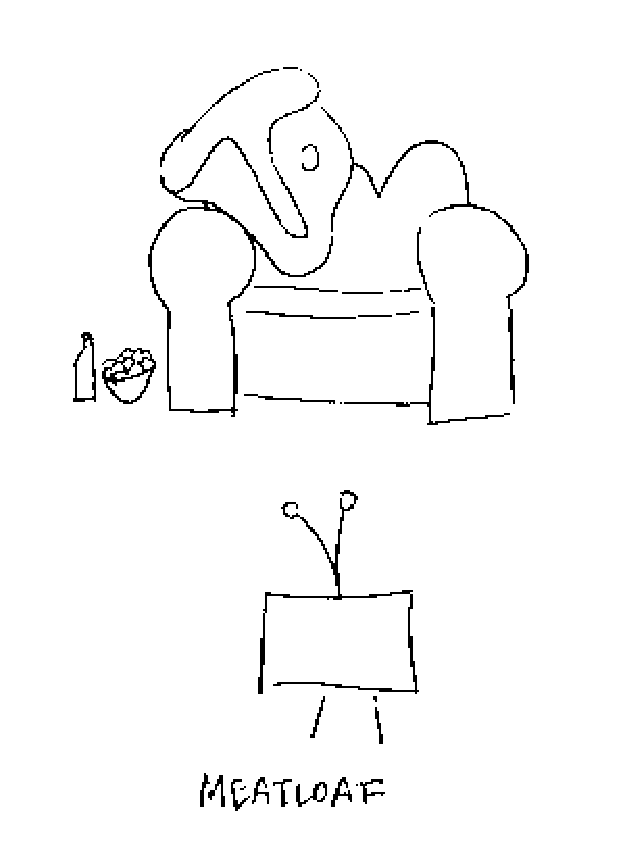
\includegraphics[scale=.5,clip]{meatloaf.ps}}

\section{Swiss Meatloaf\index{entrees!swiss meatloaf}}
\label{sec:swiss-meatloaf}

\textit{This was contributed by Joyce Evans, and is definitely ``comfort
food''! Serves 6.}
\begin{ingredients}
1 egg \\
1/2 cup evaporated milk \\
1 tsp. rubbed sage \\
1 tsp. salt \\
1/2 tsp. black pepper \\
1 1/2 lbs. lean ground beef \\
1 cup cracker crumbs (round buttery type, approx. 24) \\
3/4 cup grated Swiss cheese \\
1/4 cup finely chopped onion \\
2-3 strips bacon, cut into 1 in. pieces \\
\end{ingredients}
Preheat oven to \oven{350}. Beat the egg in a large bowl. Add evaporated milk, 
sage, salt, and pepper.  Mix together. Add beef, crumbs, 1/2 cup of the cheese
and the onion. Blend. Form into a loaf and place in a 2 quart rectangular dish.
Arrange bacon pieces on top of the loaf, and bake for 40 minutes. Sprinkle
remaining 1/4 cup cheese on top and bake 40 minutes longer. 

\section{Devilled Crabs\index{entrees!devilled crabs}}

\textit{This is from Dodge and Martha Johnson in memory of
a great southern cook, Martha Hodgkins Niepold Lamb (Kate's Grandmother).
Don't be scared by the lack of ingredient quantities. Its easy and delicious.
Just adjust until it tastes good.}
\begin{ingredients}
1 stick butter\\
2 eggs\\
a little flour and water\\
Worchestershire sauce\\
dry mustard\\
vinegar\\
pinch of sugar, salt, pepper, and MSG\\
1 lb. crab
\end{ingredients}
Preheat oven to \oven{350}.  Melt butter. Mix eggs with flour and water and add
to butter. Continue mixing and add everything else. stuff in scallop shells or
small casseroles and dot with butter and bread crumbs. Bake for 1 hour.
\begin{center}
    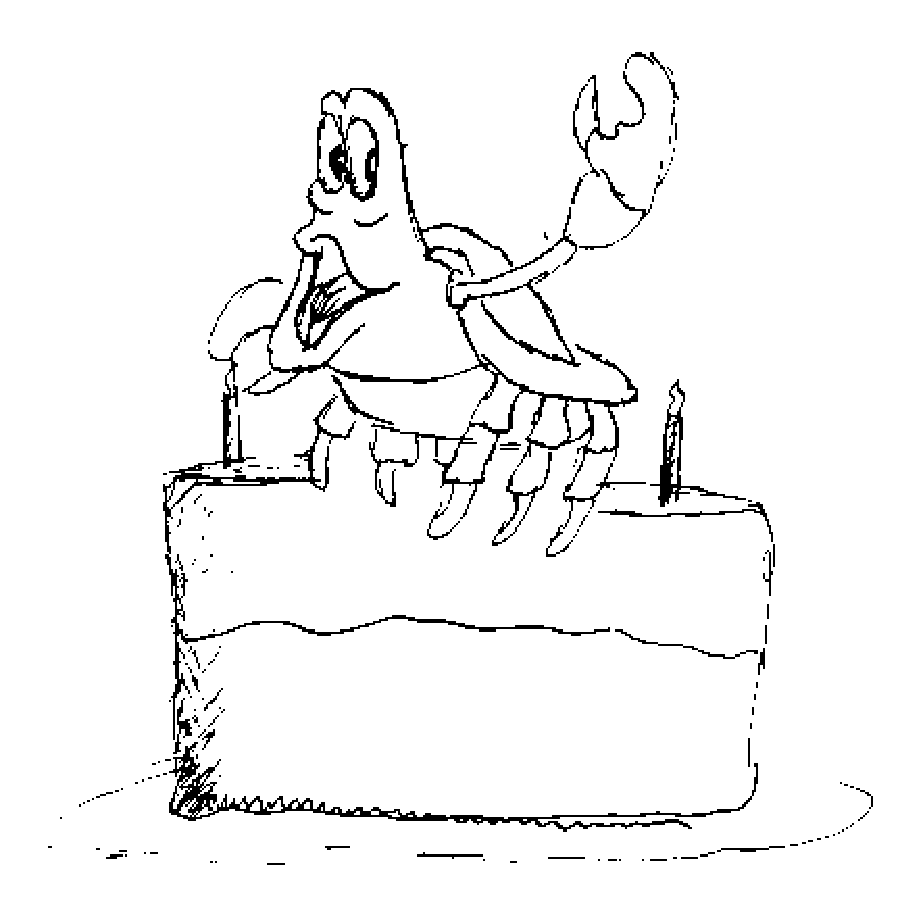
\includegraphics[width=3in,clip]{crab.ps}
\end{center}

\section{Orange Game Hens\index{entrees!Orange Game Hens}}

\textit{This is a recipe courtesy of Martha and Dodge Johnson's friends, the
Nicolsons. It's a great dish for company-especially at their house because
they are such nice people and good cooks!}
\begin{ingredients}
2 or more Cornish game hens, whole or halved\\
Joyce Chen's orange Szechuan sauce (or sub in soy sauce with orange 
concentrate)\\
2--3 Tbsp. of orange concentrate\\
several Tbsp. white wine\\
garlic powder\\
ground ginger (fresh or frozen root is best)
\end{ingredients}
Preheat oven to \oven{350}. Pour sauce, concentrate, and wine over hens. Sprinkle
with garlic powder and ginger. Cover and bake for 1 hour, and uncover last 10
minutes. Good over a bed of rice. 

\section{Chapel Hill Chicken Pie\index{entrees!Chapel Hill Chicken Pie}}

\textit{This is from Martha and Dodge, and Kate. Kate's  addition is 
only the
rosemary and measured amounts, for convenience (and my subtractions are those
nasty onions) No one cares what or how mcuh you put in, as long as you are happy.
This is one of those recipes that you put some in, then you take some out (Nana,
does this sound familiar?) This is also the kind of recipe where you vary it
based on what you like or what's sitting in the fridge! It's best when you have
leftover gravy along with meat from a past meal.}
\begin{ingredients}
2 cups chopped meat (roast lamb, beef, or chicken)\\
3--4 cubed and peeled potatoes\\
1.5--2 cups gravy or combination of stock and wine\\
2 Tbsp. flour\\ 
1 tsp. salt\\
2 tsp. pepper\\
1 Tbsp. dried parsley\\
1 tsp. garlic powder or 1 garlic clove\\
1 tsp. thyme (if using chicken or beef)\\
1 Tbsp. fresh rosemary \\
1 tsp. marjoram (if using lamb)\\
1 tsp. tarragon (if using chicken)\\
Pie Crust (\corp{Betty Crocker's} mix is good, sorry 
\corp{Duncan Hines}, you don't make one!) 
\end{ingredients}
1--2 cups each of your favorite vegetables, such as  
\begin{ingredients}
chopped carrots\\ 
green beans\\
celery\\ 
onion\\
mushrooms\\
peas\\
\end{ingredients}
Preheat oven to \oven{450}. Boil potatoes until somewhat cooked through, about
15 minutes. In a flat-ish casserole (1.5-2 qt.), layer meat, vegetables, and
potatoes. sprinlke spices over, and then flour. Add gravy mixture; adjust so
the liquid comes up about half the height of the ingredients.  Top with crust,
seal edges, and add fork holes or vents. Brown for 15 minutes, then then lower
temperature to \oven{350} and bake for 45 minutes longer. I find that I have to
cover it for the last 15 minutes or so to keep the crust from getting too brown.

\section{Pasta with Prosciutto\index{entrees!Pasta with Prosciutto}}

\textit{Martha and Dodge originally got this from the New York Times,
but it has evolved. It's
rather quick and satisfying. They say the order of tasks is a little tricky for
non-Italian cooks. Luckily, half the family  need not worry.}
\begin{ingredients}
3 cups chopped plum tomatoes\\
2-3 thinly sliced small zucchini\\
1/8-1/4 lb. prosciutto, cut into strips\\
1 tsp. salt\\
2 tsp. pepper\\
1/2 tsp. red pepper flakes (optional)\\
1 cup whipping cream
1/2 cup chopped fresh basil\\
1/4 cup grated parmesam (use the real thing not the cylinder, people)\\
1+ cloves garlic, chopped\\
1 Tbsp. olive oil\\
about 3/4 lb. pasta 
\end{ingredients}
Cook pasta. Save 1/3 cup cooking water. In frying pan, sear garlic, add
zucchini, prosciutto, salt and pepper, red pepper flakes, then tomatoes.
Stir for 2-3 minutes.  Add saved water, cream and simmer briefly. Add
pasta, basil, and parmesan, and toss. Transfer to serving dish and eat
immediately (not difficult to do!) Serves 2-3.

\section{Pasta al Cavalfiore (with Cauliflower)
\index{entrees!Pasta al Cavalfiore}}

\textit{Don sends this yummy looking dish from the Moosewood cookbook. Don says
it's good and adds ``so enough of sending pasta recipes to the Italians.''}
\begin{ingredients}
1 onion (optional if you're Kate)\\
1 cauliflower head, chopped into bite sizes\\
1 tomato\\
garlic to taste\\
2 cups grated cheese (see below)\\
1/4 cup olive oil\\
1 can tomato sauce\\
3/4 lb. pasta\\
basil, dried and some fresh too if possible\\
1 tsp. salt\\
1 tsp. pepper
\end{ingredients}
Chop the onion and garlic and saute them in 1 Tsp oil with the basil. When
onion is clear, add cauliflower and cook until tender. (Don tip: add a
handful of water, and cover to speed this along.) Add chopped tomato,
tomato sauce, salt and pepper, and simmer for about twenty minutes. During
this time, cook and drain pasta. Add the remaining olive oil to pasta
along with fresh basil and half the cheese. Don recommends the cheese be
a mixture of parmesan, romano, mozzarella, and cheddar. Spread this on a big
platter and top with the cauliflower mixture. Top with remaining cheese. Don
recommends a California gewurtstraminer ``to go with.''  Serves 2-3.

\section{Sweet and Sour Pork\index{entrees!Sweet and Sour Pork}}

\textit{Tom and Kate eat this a lot; its a ``regular''. It's 
word-for-word from a Southern Living year-end cookbook I
love (1992, if curious). Its quite delicious, and its even somewhat 
healthy.}
\begin{ingredients}
1 Tbsp. sherry\\
1 Tbsp. soy sauce\\
1 Tbsp. cornstarch\\
1 lb boneless pork, cut into cubes\\
1/4 vegetable oil, divided\\
1 clove garlic, minced\\
1 small onion (optional)\\
2 green peppers, cut into 1 in. pieces\\
1/3 cup sugar\\
1/4 cup ketchup\\\
1 Tbsp. sherry\\
2 Tbsp. soy sauce\\
2 Tbsp. white vinegar\\
1 Tbsp. cornstarch\\
1/3 cup water\\
1 8 oz. can pineapple slices in juice, each cut into about 8 pieces
\end{ingredients}
Combine first 3 ingredients, add pork, and let marinate 20 minutes (or however
long it takes to prepare everything else). Heat 2 Tbsp. oil in big frying pan.
Stir fry onion garlic, and green pepper over med-high heat until crisp tender.
Remove from skillet. Add rest of oil and cook pork until cooked through.
Stir in cooked vegetables. Combine sugar and next 6 ingredients, stirring
until cornstarch dissolves. Add to pork mixture and cook until it comes to
a boil. Add pineapple and and boil for about 1 minute. Serve over hot
cooked rice. Serves 2-3 hungry people.

\chapter{Treats}

\section{Fermina's Ginger Snaps\index{treats!gingersnaps}}

\textit{This is a super-yummy cookie recipe sent in from
Fermina.  She tells us that she always doubles this 
recipe when making a batch. Maybe the
increased amounts of ingredients help the taste factor.  Either that or we're
just gluttons.  Here's the recipe.} 
\begin{ingredients}
3/4 cup of shortening \\ 
1 cup sugar \\ 
1/4 cup light molasses \\ 
1 slightly beaten egg \\ 
2 cups flour \\ 
1/4 tsp.  salt \\ 
1 tsp.  cinammon \\ 
2 tsp. soda \\ 
1 tsp.  clove \\ 
1/2 tsp.  ginger
\end{ingredients} 
Cream shortening and sugar, add molasses
and egg.  Mix all dry ingredients.  Stir dry ingredients into creamed mixture. 
Spoon into balls. Added step for yumminess:  \textit{Drop spoonfulls into sugar
before putting on baking sheet}.  One spray of water before baking.  Bake
350$^{\circ}$ for 8 to 10 minutes.  The cookies should be split in the middle
when finished.

\section{Betsy's Chocolate Chip Poundcake\index{treats!chocolate chip pound
cake}}

\textit{This is the famous Betsy Cordova's Chocolate Chip
Cake. When she e-mailed this to use she sent a request for many treat
recipes.  What we tell her we tell all.  Send us a recipe and you get a book.  
This serves however many you feel like depending on your hunger.}
\begin{ingredients}
3 cups sugar \\ 
2 sticks butter \\ 
6 eggs \\
3 cups flour  \\
1 carton heavy whipping cream (small size) \\ 
2 Tbsp.  vanilla \\ 
1/2 bag mini chocolate chips 
\end{ingredients}
Cream butter and sugar, add 2 eggs and 1 cup flour and beat.  Add 2 eggs and 1
cup flour and beat. Add 2 eggs and 1 cup flour and beat.  Mix in vanilla and
whipping cream and add chocolate chips.

Bake in greased and floured bundt pan at 350$^{\circ}$ degrees for 60 to 75
minutes (depending on the temperature of your oven).

\vspace{2\baselineskip}
\centerline{
\includegraphics[scale=.5,clip]{pound.ps}}
\vspace{2\baselineskip}

\section{Amy's Cheesecake\index{treats!cheesecake}}

\textit{This is a holiday favorite at the Evans/Gormley households by
 Amelia Gormley.}
\begin{ingredients}
1 box Graham Craker Crumbs \\
1/2 cup sugar \\
2 Tbsp.  flour \\
1/4 tsp.  salt \\
1 pound cream cheese \\
1 tsp.  vanilla extract \\
4 eggs \\
1 cup heavy cream
\end{ingredients}
The topping ingredients are:
\begin{ingredients}
2 cups sour cream \\
3 Tbsp.  sugar \\
1 tsp.  vanilla
\end{ingredients}
Follow the directions on the Graham Craker Box for the crust.  
Use a 9$''$ spring form pan.  Press crumb mixture into the bottom 
and sides of the pan.

%\begin{wrapfigure}{r}{1.5in}
%\centerpicture 3.19in by 2.75in (pie scaled 300)
%\end{wrapfigure}
Let cream cheese soften at room temperature (or use microwave).  Mix sugar,
flour, and salt.  Add dry ingredients to cream cheese.  Cream together with low
speed beater or by hand.  Seperate eggs, save the whites in a clean bowl.  Add
yolks to cream cheese mixture and beat until smooth.  Add vanilla.  Stir in
cream.  Beat egg whites until stiff.  Fold into cream cheese mixture.  Pour on
top of crumbs.  Bake at \oven{350} for 1 hour.  Let cool.  Mix topping
ingredients.  Pour topping onto cheesecake and bake at \oven{500} for 10
minutes.  Serve with cherry, blueberry, etc. etc. toppings.

\section{Pineapple Upside-down Cake\index{treats!pineapple upside-down cake}}

\textit{Kate: On his/her birthday most kids I knew asked for chocolate cake, or
ice-cream cake,  or even cheesecake if  sophisticated. But not Tom.
Tom always begged for this somewhat unusual birthday cake. Luckily, Fermina
Evans has a great recipe for it!
Tom: I begged for it because it's delicious. Any kid would agree.}
\begin{ingredients}
1/2 cup butter \\
1/2 cup packed brown sugar \\
1 large can pineapple slices in syrup \\
1 small jar maraschino cherries
1\ 1/2 cup non packed flour (softasilk flour recommended) \\
1 cup sugar \\
2 tsp. baking powder \\
1/2 tsp. lt \\
1/3 cup soft shortening \\
2/3 cup milk \\
1 tsp. vanilla \\
1 large egg
\end{ingredients}
Melt butter with brown sugar in 9" baking pan (Fermina adds 1 Tbsp. Karo syrup
here) Arrange pineapple slices on top of syrup and place cherries in pineapple
centers or wherever they look nice. 

In mixing bowl, stir flour, sugar, baking powder and salt. Add shortening,
milk, and vanilla. Beat 2 minutes at medium speed with electric mixer. Add egg
and beat two more minutes. Pour batter over fruit. Bake at \oven{350} for
40-50 minutes. Immediately turn upside
down on serving dish (if you don't, sugar will crystallize to pan and you will
have a mess). 

\section{Chocolate Mint Brownies\index{treats!chocolate mint brownies}}

\textit{Kate: Blah blah blah chocolate blah.  Tom:  These are yummy!  My mom
makes them}.
\begin{ingredients}
1 cup sugar\\
1/2 cup butter or margarine\\
4 eggs, beaten\\
1 cup flour\\
1/2 tsp. lt\\
1 can \corp{Hershey's Chocolate Syrup} (16 oz.)\\
1 tsp. vanilla
\end{ingredients}
Mix together above ingredients and put in a greased $9''\times 13''$ pan. 
Bake at \oven{350} for 30 minutes.

The middle layer ingredients are:
\begin{ingredients}
2 cups pwedered sugar\\
1/2 cup butter or margarine\\
2 Tbsp \corp{Creme de Menthe} (preferably the green kind
\end{ingredients}
Mix and spread over cooled cake.

The glaze ingredients are:
\begin{ingredients}
1 cup chocolate chips\\
6 Tbsp butter
\end{ingredients}
Let the cake cool slightly and spread over brownies.  Chill and cut into
squares.

\section{Gooey Butter Cake\index{treats!gooey butter cake}}

\textit{A recipe from Fermi's friend Pam L.}
\begin{ingredients}
1 pkg. yellow cake mix\\
1/2 cup melted butter\\
1 egg
\end{ingredients}
The topping ingredients are:
\begin{ingredients}
8 oz. cream cheese (1 pkg.)\\
2 eggs\\
1 box powdered sugar
\end{ingredients}
Preheat oven to \oven{350}.  Mix together cake ingredients.  Pat into
$9''\times 13''$ pan.  Beat topping ingredients together for three minutes.
Pour over cake mix.  Bake for forty minutes.  Do not overbake. Top should be 
set, but not dry.

\section{Chocolate Surprise\index{treats!chocolate surprise}}

\textit{Fermi's chocolate \& angel food cake.  George's birthday favorite.}
\begin{ingredients}
32 large marshmellows\\
1/3 cup water\\
1/4 tsp. lt\\
6 oz.\ semi-sweet chocolate chips\\
heavy whipping cream and sugar\\
1/4 tsp. vanilla
\end{ingredients}
\begin{wrapfigure}{l}{2.0in}
\centerline{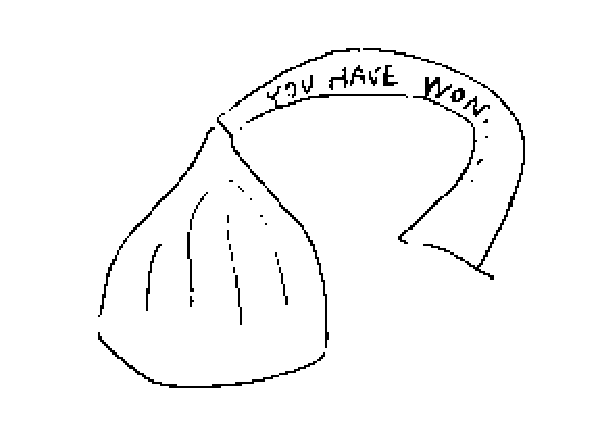
\includegraphics[width=1.8in,clip]{kiss.ps}}
\end{wrapfigure}
In sauce pan melt marshmellows, water, and salt.  Add chocolate bits.  Stir
until melted.  Let cool.

Whip 1 cup whipping cream.  Pour chocolate over cream and fold together.

Take a store brought or home make angel food cake.  Cut off entire top 1$''$
layer.  WIth spoon dig a tunnel in remaining cake.  Fill with chocolate
surprise.  Replace top layer.

Sprinkle cake with powdered sugar or frost with whipped cream (1 cup heavy
cream beaten with 1 Tbsp. sugar until stiff).  

\section{Tiramisu\index{treats!tiramisu}}

\textit{Mimi Horne brings us this delicious treat from an
Italophile Brazilian Yale Art History Professor friend, Ester da Costa Meyer.
Those in less gastro-enlightened regions might need to replace the mascarpone
with cream cheese and cream, and the Marsala with perhaps port or sherry. }
\begin{ingredients}
2-3 pkgs (about 24-30) lady fingers (boudoirs) \\
3 cups mascarpone (or part creme fraiche, part carre frais mushed together)\\
3 egg yolks \\
1/3 cup sugar \\
2 cups strong coffee \\
1/2 cup or more Marsala wine \\
1/2 cup cocoa
\end{ingredients}
Prepare coffee and mix with Marsala. One at a time, dip lady fingers in mixture
briefly, then lay them in a row in an approx. $10''\times 18''\times 2 1/2''$
deep serving dish.
Cut some to fit the remaining space in dish so that the bottom is
completely covered. Mix sugar, egg yolks and mascarpone/cream. Spread
about half the mixture over the first layer of cookies to cover completely.
Dip more lady fingers in coffee/Marsala and lay them over cream to form the
next layer; cover remaining cream mixture. Dust the top thoroughly with cocoa;
chill overnight or for several hours before serving. More cocoa may be added
before serving. The texture can be made lighter by beating the egg whites and
folding them into the mascarpone mixture, which also increases the amount.
Serves 6-8.

\section{Tortelettes\index{treats!Tortelettes}}

\textit{Another Nonnie/Grandpatty and Joy of Cooking original. Niepold kids
remember Christmas at Lee St. when they eat Tortelettes and California dates
stuffed with Georgia Pecans and rolled in confectioners' sugar.}
\begin{ingredients}
1 grated lemon rind\\
1 cup sugar\\
3/4 cup butter\\
2 egg yolks \\
1/2 cup bread flour \\
1 cup blanched and shredded almonds or pecan pieces \\
1/3 cup sugar \\
1 tsp. cinnamon\\
1/4 tsp. nutmeg\\
1/8 tsp. salt\\
1 egg white\\
1 Tbsp water
\end{ingredients}
Preheat oven to \oven{375}. Grate lemon into sugar. Cream sugar with butter and
beat in the egg yolks one at a time. Add flour gradually to make a stiff
dough. Pinch off about a teaspoonful of dough at a time. Roll it into a ball
and flatten on cookie sheet until very thin. Prepare nuts and combine with
next 4 ingredients (spices). Beat the egg white and water together slightly.
Brush the cakes with the egg white mixture, then sprinkle nut/spice mixture
and bake until light brown.  

\section{Lime Cream Pie\index{treats!Lime Cream Pie}}

\textit{Kate got this recipe from Edie, a receptionist at Bryn Mawr College
with southern cooking blood. 
It's very easy and delicious, especially after a rich
meal. It's cool, refreshing, and slides right down.}
\begin{ingredients}
1 Graham Cracker Pie Crust\\
3 egg yolks\\
2 2/3 cups sweetened condensed milk (2 cans)\\
1 cup plus 2 Tbsp lime juice (about 7 limes if you're squeezing)\\
2 tsp. grated lime zest\\
1 attractive lime
\end{ingredients}
Lightly whisk egg yolks in mixing bowl. Pour in
condensed milk and whisk until completely blended.  Add lime juice and zest and
whisk to blend. Gently pour filling into pie crust shell and smooth over top.
Refrigerate for at least 4 hours (don't skimp or it will be soup!). Slice
the attractive lime paper thin to garnish. I like to slice into
half-circles and create a pinwheel pattern around the center. 


\backmatter

\chapter{Family Information}

\section{List of Contributors}

\begin{enumerate}
\item Betsy and Rich Cordova, \textit{411 Arrowhead Trail, Sinking Spring
PA  19608}.  Rich is in med. school so they're on the move.  This is the
easiest place to find out where they are.
\item Angelo and Evelina DeLellis, \textit{238 Faust Road,
Sinking Spring, PA 19608}.
\item George, Sr. and Mickey Evans, \textit{1822 Village Lane,
Bentley Village, Naples FL, 33963}.
\item Fermina, Geo, and Kate Evans, \textit{411 Arrowhead Trail, 
Sinking Spring PA, 19608.}
\item Steve, Joyce, and Scott Evans, \textit{c/o Steve Evans, 1890 Madison
 Ave., Cincinnati, OH 45206.} Scott is actually in school at Ohio State.
\item Tom and Kate Evans, \textit{3515 Pleasantdale Rd. 332, 
Atlanta GA, 30340.}
\item Amy and Ed Gormley, Lauren Anton, \textit{5 Knollwood Drive,
Sinking Spring, PA 19608}.
\item Paul and Mimi Horne, \textit{28 ave. R Poincar\'{e}, 75116
Paris, France}.
\item Rich, Jen, Julian, and Nicholas King, \textit{Margrietlaan 15,
6165 Cr Geleen, The Netherlands}.
\item Don and Lil Johnson, \textit{115 Norris Road,
Wilmington, DE 19883.}
\item Donald Johnson, III, \textit{121 Warwick Street SE 1, 
Minneapolis, MN 55455}.  Make sure you add the
III behind Don's name, he loves that.
\item David Lindquist and Jen Tidy, \textit{236 South Prosect Street 1,
Burlington, VT  05401}.
\end{enumerate}

\section{Family Trees}

We realized while writing this recipe book that many of you don't know
people from either Tom's or Kate's extended families.  To resolve this
Tom proposed a biblical-style section, ie. Donald begot Dodge who was the
Father of Kate...  Kate, on the other hand hated that format, and, for
once, Tom agreed.  Therefore, we settled on family trees because they
remind Tom of Feynman Diagrams and because Kate thinks they look like
something having to do with weather.  Anyway, these are meant for people
from one side of the hill to see who is related to who on the other side.
They are not conclusive and only reflect the situation as it is now.
\vspace*{\fill}
\pagebreak
\begin{center}
\includegraphics[angle=90,height=8.5in,clip]{ktree.eps}
\end{center}
\pagebreak
\centerline{
\includegraphics[angle=90,height=8.5in,clip]{ttree.eps}}

\printindex
\end{document}

